\documentclass[11pt,a4paper]{article}
\usepackage[a4paper,top=14mm,bottom=14mm,left=15mm,right=15mm]{geometry}
\usepackage[T1]{fontenc}
\usepackage{amsmath}
\usepackage{amssymb}
\usepackage{array}
\usepackage{multicol}
\usepackage{tikz}
\usetikzlibrary{arrows.meta}

% ================================================================
% Probability: revision questions.
%
% Two pages of questions, in black and white, with a heading for each
% topic on the Maths Revision topic list in the same order. Each topic
% has a few short questions that start easy, with a diagram only where
% a question uses one, and the sheet ends with some problem solving.
% There are no key facts or worked examples on the sheet: the methods
% are in the worked solutions and the revision guide. Questions are
% numbered through the sheet so that the answer key and the worked
% solutions can refer to them.
% ================================================================

\pagestyle{empty}
\setlength{\parindent}{0pt}
\setlength{\parskip}{2pt}
\setlength{\columnsep}{9mm}

% A topic from the revision list.
\newcommand{\topic}[1]{\par\addvspace{9pt}{\bfseries #1}\par\nobreak\vspace{2pt}}

% Questions are numbered through the whole sheet.
\newcounter{qn}
\newcommand{\q}{\par\addvspace{5pt}\stepcounter{qn}\hangindent=1.6em\hangafter=1\noindent
  \makebox[1.6em][l]{\textbf{\theqn}}}

% \venn{<left set>}{<right set>}{<left only>}{<both>}{<right only>}{<outside>}
% The last argument is drawn as it stands, to place the outside
% region's contents anywhere around the circles.
\newcommand{\venn}[6]{%
  \begin{tikzpicture}[x=1mm,y=1mm]
    \draw (0,0) rectangle (66,34);
    \node[anchor=north west] at (0,34) {$\xi$};
    \draw (24,17) circle (13.5);
    \draw (42,17) circle (13.5);
    \node at (10,30) {$#1$};
    \node at (56,30) {$#2$};
    \node[align=center] at (17.5,17) {#3};
    \node[align=center] at (33,17) {#4};
    \node[align=center] at (48.5,17) {#5};
    #6
  \end{tikzpicture}}

% \freqtree{<total>}{<group>}{<n>}{<group>}{<n>}{<leaf>}{<leaf>}{<leaf>}{<leaf>}
% A frequency tree drawn left to right. The two outcomes on the right
% hand branches are named by \leafa and \leafb.
\newcommand{\leafa}{}
\newcommand{\leafb}{}
\newcommand{\freqtree}[9]{%
  \begin{tikzpicture}[x=1mm,y=1mm,
      box/.style={draw,minimum width=9mm,minimum height=5.5mm,inner sep=1pt},
      lab/.style={font=\small,inner sep=1pt}]
    \node[box] (r) at (0,0) {#1};
    \node[box] (u) at (18,10) {#3};
    \node[lab,above] at (u.north) {#2};
    \node[box] (d) at (18,-10) {#5};
    \node[lab,below] at (d.south) {#4};
    \node[box] (uu) at (37,14.5) {#6};
    \node[box] (ud) at (37,5.5) {#7};
    \node[box] (du) at (37,-5.5) {#8};
    \node[box] (dd) at (37,-14.5) {#9};
    \foreach \n in {uu,du}{\node[lab,right] at (\n.east) {\leafa};}
    \foreach \n in {ud,dd}{\node[lab,right] at (\n.east) {\leafb};}
    \draw (r.east) -- (u.west) (r.east) -- (d.west);
    \draw (u.east) -- (uu.west) (u.east) -- (ud.west);
    \draw (d.east) -- (du.west) (d.east) -- (dd.west);
  \end{tikzpicture}}

\begin{document}
% Ragged right, without \raggedright, which would make \\ end the
% paragraph and lose the hanging indent of a question's later lines.
\setlength{\rightskip}{0pt plus 4em}

{\Large\bfseries Probability}\hfill{\large Revision questions}
\par\vspace{2pt}\hrule\vspace{4pt}

\begin{multicols}{2}

% ----------------------------------------------------------------
\topic{Writing probabilities as fractions, decimals and percentages}
\q A bag holds 4 green (G), 6 yellow (Y) and 10 white (W) sweets. One sweet is taken at random. Write P(green) as a fraction, a decimal and a percentage.\\[4pt]
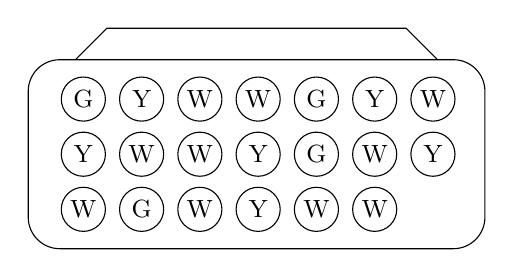
\begin{tikzpicture}[x=1mm,y=1mm]
  \draw[rounded corners=4mm] (0,0) rectangle (58,24);
  \draw (6,24) -- (10,28) -- (48,28) -- (52,24);
  \foreach \l [count=\i from 0] in {G,Y,W,W,G,Y,W,Y,W,W,Y,G,W,Y,W,G,W,Y,W,W}{
    \pgfmathtruncatemacro{\r}{\i/7}
    \pgfmathtruncatemacro{\c}{mod(\i,7)}
    \draw (7+\c*7.4,19-\r*7) circle (2.8);
    \node[font=\small] at (7+\c*7.4,19-\r*7) {\l};}
\end{tikzpicture}
\q The probability that a train is late is 0.12. What is the probability that it is not late?
\q The table shows the probabilities of a spinner landing on each colour. Find the probability that it lands on yellow.\\[4pt]
{\renewcommand{\arraystretch}{1.5}%
\begin{tabular}{|l|c|c|c|c|}\hline
Colour & Red & Blue & Green & Yellow\\\hline
Probability & 0.3 & 0.25 & 0.15 & \\\hline
\end{tabular}}

% ----------------------------------------------------------------
\topic{Listing outcomes systematically}
\q A caf\'e sells three starters: soup (S), melon (M) and prawns (P). It sells two mains: fish (F) and curry (C). List all the possible meals of one starter and one main.
\q Spinner A is numbered 1, 2, 3, 4. Spinner B is numbered 1, 2, 3. Both spinners are spun, and the two scores are multiplied.\\
(a) Copy and complete the sample space diagram.\\
(b) Find the probability that the answer is even.\\[4pt]
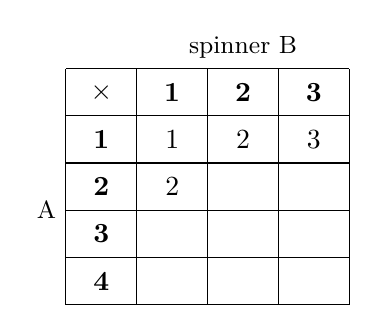
\begin{tikzpicture}[x=9mm,y=6mm]
  \draw[step={(1,1)}] (0,-4) grid (4,1);
  \node at (0.5,0.5) {$\times$};
  \foreach \b in {1,2,3}{\node at (\b+0.5,0.5) {\textbf{\b}};}
  \foreach \a in {1,...,4}{\node at (0.5,-\a+0.5) {\textbf{\a}};}
  \foreach \b in {1,2,3}{\node at (\b+0.5,-0.5) {\b};}
  \node at (1.5,-1.5) {2};
  \node[above] at (2.5,1) {\small spinner B};
  \node[left] at (0,-2) {\small A};
\end{tikzpicture}

% ----------------------------------------------------------------
\topic{Expected results}
\q A fair coin is flipped 300 times. How many heads would you expect?
\q The probability that a bus is late is 0.08. On how many of 250 journeys would you expect the bus to be late?

% ----------------------------------------------------------------
\topic{Experimental probability}
\q A dice is rolled 200 times. The table shows the results.\\[4pt]
{\renewcommand{\arraystretch}{1.5}%
\begin{tabular}{|l|c|c|c|c|c|c|}\hline
Score & 1 & 2 & 3 & 4 & 5 & 6\\\hline
Frequency & 31 & 35 & 30 & 36 & 33 & 35\\\hline
\end{tabular}}\\[4pt]
(a) Find the relative frequency of rolling a 4.\\
(b) Do the results suggest that the dice is fair? Explain your answer.
\q Jo flips a coin 20 times and gets 14 heads. Kai flips the same coin 500 times and gets 260 heads. Whose results give the better estimate of the probability of heads? Write down this estimate.


% ----------------------------------------------------------------
\topic{Frequency trees}
\q 120 people visited a museum. 70 of them were adults. 45 of the adults bought a guidebook. 20 of the children bought a guidebook.\\
(a) Copy and complete the frequency tree.\\
(b) A visitor is chosen at random. Find the probability that they bought a guidebook.\\[4pt]
{\renewcommand{\leafa}{Book}\renewcommand{\leafb}{No book}%
\freqtree{120}{Adults}{}{Children}{}{}{}{}{}}

\end{multicols}

\newpage

\begin{multicols}{2}

% ----------------------------------------------------------------
\topic{Venn diagrams}
\q There are 50 pupils in a year group. 28 study French (F), 19 study Spanish (S), and 8 study both.\\
(a) Copy and complete the Venn diagram.\\
(b) A pupil is chosen at random. Find the probability that they study neither language.\\[4pt]
\venn{F}{S}{}{}{}{}
\q The Venn diagram shows the numbers from 1 to 15. A is the even numbers and B is the square numbers. One of the numbers is chosen at random. Find\\
(a) P($A\cap B$), the probability that it is in A and B\\
(b) P($A\cup B$), the probability that it is in A or B or both\\
(c) P($A'$), the probability that it is not in A.\\[4pt]
\venn{A}{B}{\hspace*{2mm}2\enspace 6\\[1pt]\hspace*{2mm}8\enspace 10\\[1pt]\hspace*{2mm}12\enspace 14}{4}{1\\[2pt]9}%
  {\node at (4,17) {3}; \node at (62,17) {5}; \node at (4,4) {7}; \node at (62,4) {11};
   \node at (33,31.3) {13}; \node at (33,2.7) {15};}

% ----------------------------------------------------------------
\topic{Conditional probability with Venn diagrams}
\q The Venn diagram shows 60 people, and whether they own a cat (C) or a dog (D).\\[4pt]
\venn{C}{D}{14}{10}{21}{\node at (60,4) {15};}\\[2pt]
(a) Find the probability that a person chosen at random owns a dog.\\
(b) Given that a person owns a dog, find the probability that they also own a cat.
\q Use your Venn diagram from question 11. Given that a pupil studies French, find the probability that they also study Spanish.


% ----------------------------------------------------------------
\topic{Problem solving}
\q A bag holds red and blue counters in the ratio $3:5$. Two more red counters are put in the bag. Now the probability of taking a red counter is $\frac12$. How many counters were in the bag at the start?
\q A spinner has 5 equal sections, each coloured red, blue or green. The probability of red is 0.4, and the probability of blue is twice the probability of green. Draw the spinner.
\q Sam rolls a dice 6 times and never gets a 6. He says, ``The dice must be biased.'' Is Sam right? Explain your answer.

\end{multicols}

\end{document}
